\section{Comportement}
\label{sec:Comportement}
Concernant les blessures préalablement observées lors du stage de B. SOMON, aucune n'a pu être à nouveau visualisée durant mon stage. Les animaux ont cependant été qualifiés de "plus sensible à leurs environnement que la normale" par les animaliers en charges de ceux-ci. On peut donc penser que durant le stage précédent, comme l'animalerie n'était pas la même, les animaux étaient soumis à un stress plus importants, et adoptaient en réponse à ce stress un comportement d'automutilation.

\section{Structure du cerveau}
\label{sec:NisslResultat}
La coloration de Nissl, ici à base de Crésyl violet, est un marquage classique du tissu nerveux avec une molécule basique, qui marque particulièrement l'acide nucléique (\acrshort{adn} et \acrshort{arn}) des cellules car basophile (ces structures au microscope prennent le nom de "Corps de Nissl'). Ce marquage est important sur les neurones, riches en \gls{re} rugueux, et donc avec une grande quantité d'\acrshort{arn}. Cette coloration permet ainsi de mettre en évidence les motifs des différentes structures cellulaires au sein du tissu nerveux.

Afin de visualiser si la mutation \mcrd altérait l'organisation structurale du cerveau, une coloration de Nissl a été réalisée sur 4 individus : 2 souris mutantes et 2 souris sauvages (1 mâle et 1 femelle pour chaque groupe) (\cref{fig:NisslResultat}). Ce marquage a permis de mettre en évidence que la mutation de \gls{musk} ne modifiait pas de manière visible l'organisation du cerveau, à la fois chez les souris femelles (\cref{fig:FemWTNissl,fig:FemMutNissl}) et mâles (\cref{fig:MaleWTNissl,fig:MaleMutNissl}). 

\begin{figure}[h] %Figure Nissl Résultats
	\begin{center}
		\begin{subfigure}[h]{0.49\textwidth}%F437 WT Nissl 33 l2.tif
			\caption{}
			\label{fig:FemWTNissl}
			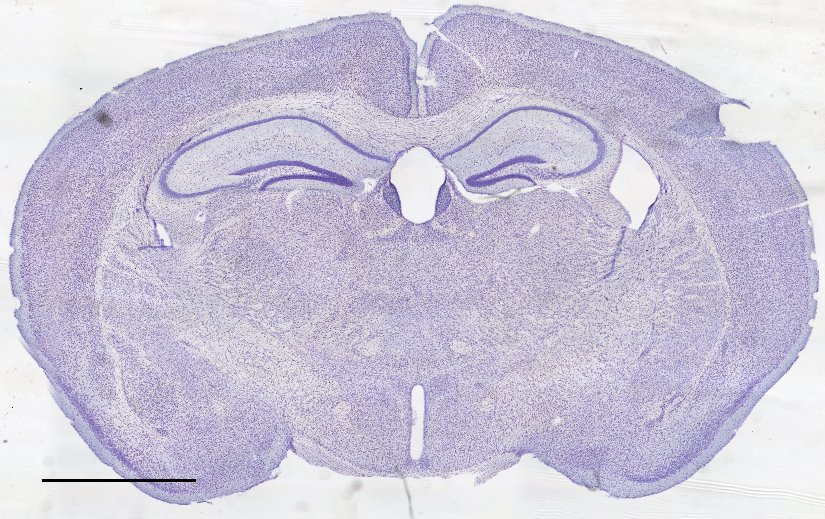
\includegraphics[width=\textwidth]{./Images/Nissl/FemWT.jpg}
		\end{subfigure}
		\begin{subfigure}[h]{0.49\textwidth}%F435 Mut Nissl 38.tif
			\caption{}
			\label{fig:FemMutNissl}
			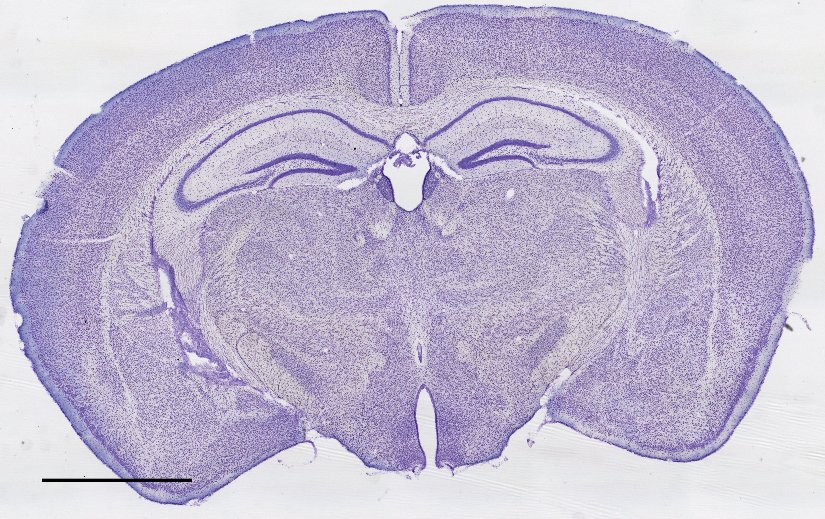
\includegraphics[width=\textwidth]{./Images/Nissl/FemMut.jpg}
		\end{subfigure}
		\begin{subfigure}[h]{0.49\textwidth}%M2 WT Nissl #031.tif
			\caption{}
			\label{fig:MaleWTNissl}
			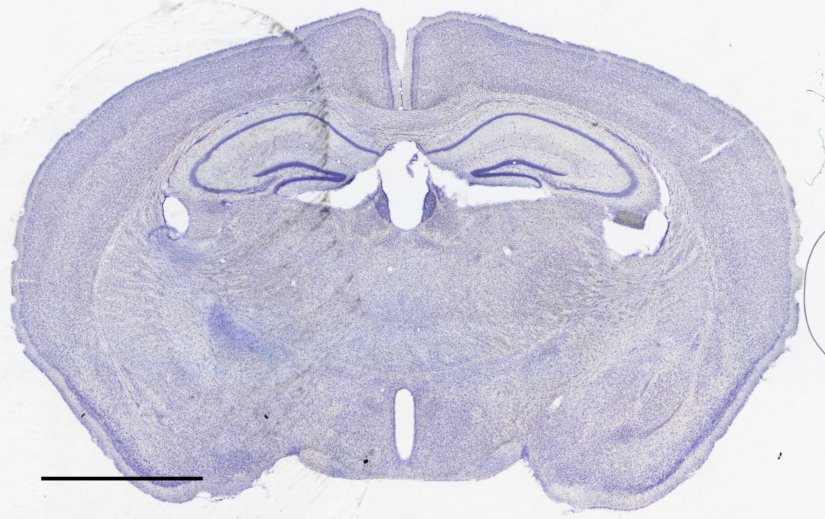
\includegraphics[width=\textwidth]{./Images/Nissl/MaleWT.jpg}
		\end{subfigure}
		\begin{subfigure}[h]{0.49\textwidth}%M442 Mut Nissl lame 3 36.tif
			\caption{}
			\label{fig:MaleMutNissl}
			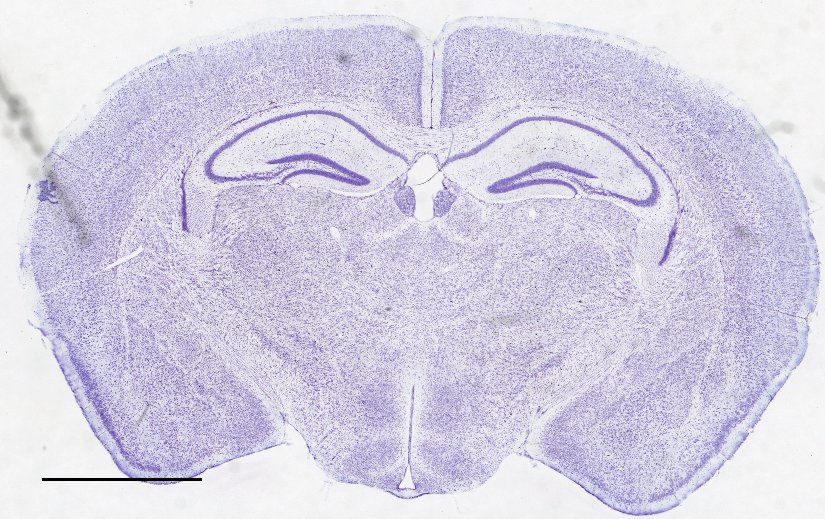
\includegraphics[width=\textwidth]{./Images/Nissl/MaleMut.jpg}
		\end{subfigure}
	\end{center}
	\caption{Pas de modifications structurelles observées chez les mutants.}
	\descfig{Coloration de Nissl sur : \subref{fig:FemWTNissl} Femelle sauvage, \subref{fig:FemMutNissl} Femelle mutante, \subref{fig:MaleWTNissl} Mâle sauvage, \subref{fig:MaleMutNissl} Mâle mutant. Images représentatives de coupes réalisées au niveau de l'hippocampe. Âge moyen des souris : 30 jours. Barre d'échelle : 2 mm.}
	\label{fig:NisslResultat}
\end{figure}
%\FloatBarrier

\section{Immunomarquage}
\label{sec:IHC}

\subsection{\acrshort{neun}}
\label{ssec:neun}
\Acrshort{neun} est un marqueur du  corps cellulaire et des noyaux de presque tout les neurones, couramment utilisé \cite{Guselnikova2015}. Ce marquage à été utilisé afin de vérifier la distribution et le nombre des neurones au niveau de l'hippocampe des souris \mcrd était perturbée ou non.

\subsection{\acrshort{musk} et \acrshort{gfap}}
\label{ssec:musk}
Après avoir observé l'organisation neuronale du cerveau de souris, j'ai voulu observé les régions du cerveau qui exprimaient \gls{musk}. Pour cela, j'ai eu recours à des techniques d'immunomarquages. Malgré le fait que le niveau d'expression de \gls{musk} soit considéré comme faible dans le tissu nerveux, j'ai quand même pu observé un marquage de cette protéine dans diverses régions discrètes du cerveau : Hippocampe (couche radiaire et moléculaire principalement), Corps calleux, Habenula, Fasciculus retroflexus, Capsule interne, Noyau caudé, 3ème ventricule ventrale. \todo{fig avec schéma localisation ?}.

Dans ces régions, le marquage prenait la forme de prolongement cellulaires, qui rappelait ceux des astrocytes. Afin d'étudier cette hypothèse, un co-marquage entre \gls{musk} et \acrshort{gfap}, un marqueur des astrocytes a été réalisé.

Pour réaliser le marquage de \acrshort{gfap}, deux anticorps différents ont été utilisés. Le premier, fourni d'abord par l'équipe de C. AGULHON, provient de chez Millipore-Merck (\cref{table:Ac}, ref. MAB360) et fonctionne correctement. Le second anticorps, provenant de chez Abcam (\cref{table:Ac}, ref. ab4648) et commandé suite à une indisponibilité du premier anticorps, s'est révélé inefficace à différentes concentrations testées ($1{:}100$, $1{:}50$). Cependant, le premier anticorps a put être à nouveau commandé pour la suite des expériences.

\section{Immunoprécipitation}
\label{sec:IPresultat}
Afin de confirmer la détection de \gls{musk} dans diverse région du cerveau, une immunoprécipitation suivie d'un \gls{wb} a été réalisée sur l'hippocampe, le cervelet et le cortex de trois souris C57Bl/6 sauvage. Un \gls{wb} de \gls{musk} a déjà été décrit sur des diverses structures du cerveau \cite{Garcia-Osta2006}, mais à partir d'extrait total. Durant son stage, B. SOMON a tenté de réaliser un \gls{ip} suivi d'un \gls{wb}, mais sans obtenir de résultats probant. Ici, la principale modification apportée au protocole précédemment utilisée par cette étudiante est l'utilisation de tampon RIPA (adjonction de déoxycholate de sodium et de \acrshort{sds} dans le tampon) qui permet une meilleure lyse et une meilleure préservation des protéines lors de l'extraction.

\section{Expression de \gls{musk}}
\label{sec:ExpressionMuSK}
Il est intéressant de connaître le niveau d'expression de la protéine \gls{musk} dans le cerveau, afin de voir si la mutation allait impactée l'expression de la protéine. Pour cela, j'ai eu recours à la technique de \gls{qpcr} sur trois structures différentes : le cervelet, et l'hippocampe gauche ou droit. En effet, des résultats très préliminaire dans le laboratoire chez des 2 souris de souche C57Bl/6 (1 mâle et 1 femelle) avait montrée une légère différence d'expression selon le coté du cerveau étudié. De plus, on retrouvait également une différence entre des individus de sexe opposé. Il était donc nécessaire de reprendre cette technique chez un plus grand nombre d'animaux afin de confirmer ou non ces tendances.